\documentclass[article, 11pt]{IEEEtran}   %Document is an article, 11 pt font, and follows IEEE format
\usepackage{hyperref}         %Use hyperref package (for hyperlinks)
\usepackage{graphicx}         %Use graphicx package (for images)
\usepackage{float}            %Use float package (allows you to place images more easily)
%\usepackage{gensymb}          %Use gensymb package (generic symbols)
\usepackage{amsmath}          %Use amsmath package (for optimized math formulas)
\usepackage{tikz}             %Use tikz package (for creating graphics)
\usepackage{pgfplots}         %Use pgfplots package (for creating graphics)
\usepackage{pgfplotstable}    %Use pgfplotstable (for linear regression)
\usepackage[spanish]{babel}


\begin{document}
%
% paper title
% Titles are generally capitalized except for words such as a, an, and, as,
% at, but, by, for, in, nor, of, on, or, the, to and up, which are usually
% not capitalized unless they are the first or last word of the title.
% Linebreaks \\ can be used within to get better formatting as desired.
% Do not put math or special symbols in the title.
\title{Proyecto 1\\Aplicaciones de EDO}

% author names and affiliations
% use a multiple column layout for up to three different
% affiliations
\author{
	\IEEEauthorblockN{Juan José Rivera Román - 20002802\\Mario Esteban Ponce Contreras - 21000508}
	\IEEEauthorblockA{\\Universidad Galileo\\Guatemala, Guatemala }
}

% make the title area
\maketitle

% As a general rule, do not put math, special symbols or citations in the abstract
\begin{abstract}
Al momento de trabajar con ecuaciones diferenciales de primer orden, no siempre es posible expresar la solución de manera explícita o ímplicita, aun cuando sea posible demostrar que dicha solución existe. En esos casos, una forma de expresar la solución a una ecuacion diferencial es por medio de algún método numérico. En este proyecto se estudia y aplica el método de Runge-Kutta, uno de los métodos numéricos más precisos.
\end{abstract}

\section{Introducci\'on}
En este proyecto se pone en práctica lo aprendido en el curso de ecuaciones diferenciales ordinarias, los distintos tipos de métodos para encontrar las soluciones generales y particulares, además, se explorará el método de aproximación de Runge-Kutta que permite aproximar la solución a una ecuación diferencial de primer orden con valores iniciales $y\prime=f(x, y), y(x_o)=y_o$.

El objetivo principal del proyecto es entender y aplicar el método de aproximación de Runge-Kutta, comparar los resultados con el método analítico estudiado en clase y comprobar la presición del método para la resolución de ecuaciones diferenciales dados ciertos valores iniciales.

\section{Procedimiento}
Se inició la práctica investigando en distintas fuentes el método de Runge-Kutta, cómo utilizarlo y las condiciones que deben cumplir para aplicar el método. Luego se procedió a abstraer el método en código de programación para facilitar la realización pruebas que permitan validar el correcto funcionamiento del algoritmo aplicado. Finalmente, se diseñó e implementó una interfaz de usuario para que cualquier usuario pueda hacer uso del algoritmo sin conocimiento previo en programación.

\subsection{Materiales}
\begin{itemize}       							%Creating an unordered list
\item Computadora con Visual Studio Code y procesador de 1.80GHz mínimo.
\item Software: Nodejs, npm y Vue-cli.
\end{itemize}

\subsection{Diagrama de flujo del proyecto}

\begin{figure}[H]									%Creating a figure with caption
\centering
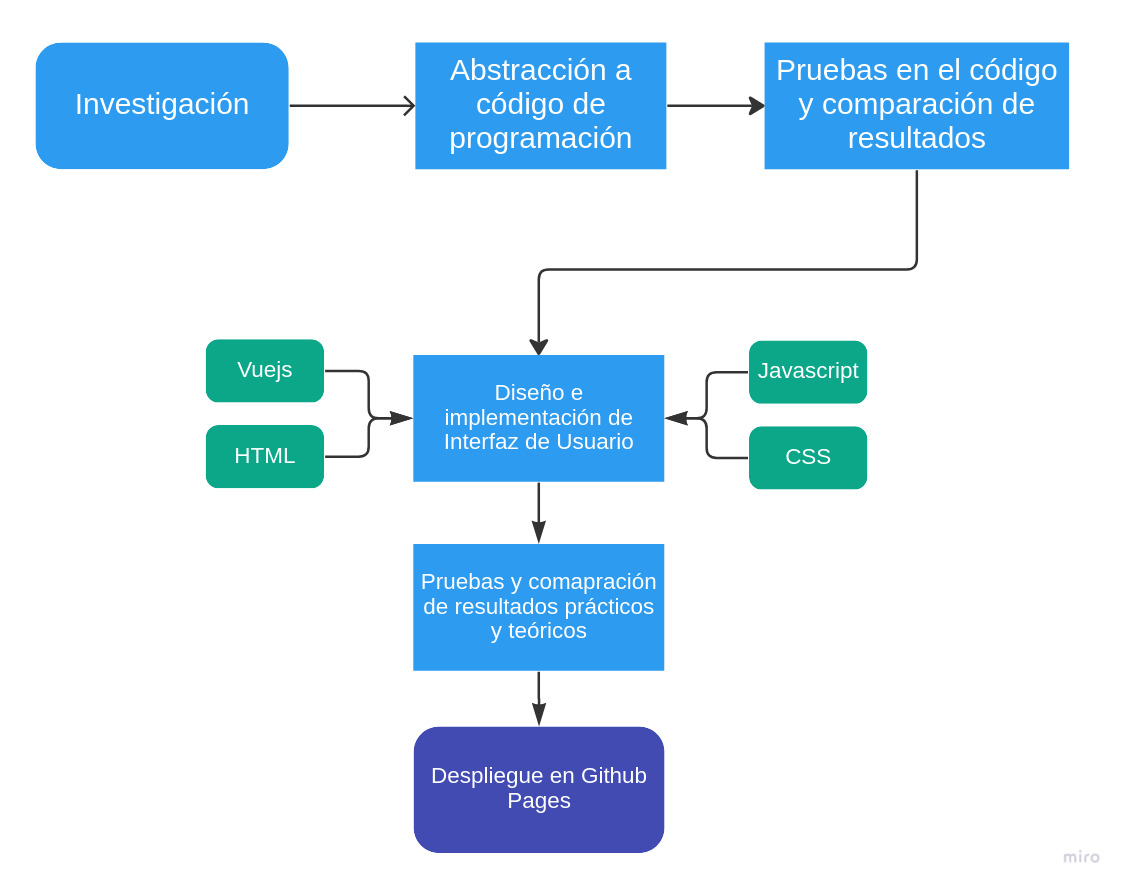
\includegraphics[scale=0.2]{flujoDeProyecto}%Inserting graphic file (in same directory)
\caption{Diagráma de flujo del proyecto}\label{diagram1}  %Captioning the graphic file
\end{figure}

\subsection{Pasos del procedimiento}        		
Siguiendo el algoritmo de aproximación del método de Runge-Kutta:
\begin{enumerate}						%Creating an ordered list
	\item Se definen la ecuación $y\prime=f(x, y)$ y sus valores iniciales $x_o$  y $y(x_o)$ además de definir el tamaño del paso $h$ entre $x_n$ y $x_{n-1}$
	\item Dependiendo del orden del método a utilizar, se calcula determinado número de términos que forman parte del promedio ponderado con el que se forma el polinomio de Taylor que se utiliza para aproximar la solución.
\end{enumerate}

\vspace{1em}

Para el métdo de primer orden:
\begin{equation}
	y_{n+1}=y_n+hf(x_n, y_n)
\end{equation}

Para el método de segundo orden:
\begin{equation}
y_{n+1}=y_n+\frac{h}{2}(k_1+k_2)
\end{equation}

Donde:
\begin{gather*}
k_1=f(x_n,y_n)\notag\\
k_2=f(x_n+h,y_n+hk_1)
\end{gather*}

Para el método de cuarto orden: 
\begin{equation}
y_{n+1}=y_n+\frac{h}{6}(k_1+2k_2+2k_3+k_4)
\end{equation}

Donde:
\begin{gather*}
k_1=f(x_n, y_n)\notag\\
k_2=f(x_n+\frac{1}{2}h, y_n+\frac{1}{2}hk_1)\\
k_3=f(x_n+\frac{1}{2}h, y_n+\frac{1}{2}hk_2)\\
k_4=f(x_n+h, y_n+hk_3)
\end{gather*}

Finalmente, se compararon los resultados obtenidos por medio del método analítico con los resultados obtenidos por medio del método de Runge-Kutta de diferente orden. En general, la aproximación es mucho mejor al aumentar el grado del método, y gráficamente, es mucho más fácil apreciar la presición del la aproximación en cuanto menor sea el paso $h$ entre cada iteración.

\section {Resultados}
\subsection{Prueba 1}
\begin{table}[H]
\centering
\caption{Datos para la prueba 1}
\label{DataTable1}
\begin{tabular}{|c|c|}
\hline
Variable & Valor inicial \\
\hline
EDO & $y\prime=x+1-y$\\
h & 0.25\\  
$y(0)$ & 0\\
x & 1\\
Solución & $y(x)=x$\\
\hline   
\end{tabular}
\end{table}

\begin{table}[H]
\centering
\caption{Resultados de la prueba 1}
\label{DataTable2}
\begin{tabular}{|c|c|c|c|c|c|}
\hline
$x_n$ & $k_1$ & $k_2$ & $y_n$ & Valor real & \% de error \\
\hline
0.00 & 0.0000 & 0.0000 & 0.0000 & 0.0000 & 0.00\%\\
0.25 & 1.2500 & 1.1875 & 0.3046 & 0.2500 & 21.88\%\\
0.50 & 1.0265 & 1.2356&1.2356 & 1.4567 & 1.8946\\
0.75 & 1.0265 & 1.2356&1.2356 & 1.4567 & 1.8946\\
1.00 & 1.0265 & 1.2356&1.2356 & 1.4567 & 1.8946\\
\hline   
\end{tabular}
\end{table}

\newpage

\subsection{Graficas}
\begin{figure}[H]
\centering
\begin{tikzpicture}
\begin{axis}[
   title=Scatterplot of Circle Quantities,	%Title of graph
   xlabel={diameter (cm)},					%label the x-axis
   ylabel={circumference (cm)},				%label the y-axis
   legend pos=south east,					%put slope legend in bottom right corner
]
\addplot[blue, only marks] table {CircleData.dat};	%plot points from data table
\addplot [red] table [y={create col/linear regression={y=y}}]   %best fit line
        {CircleData.dat};
       
\addlegendentry{slope=$\pgfmathprintnumber{\pgfplotstableregressiona}$}        
        %show slope value
\end{axis}
\end{tikzpicture}
\caption{Ejemplo de gr\'afica}\label{diagram1}   %caption the graph
\end{figure}

\section{Discusi\'on / An\'alisis}
En esta secci\'on se discute los resultados obtenidos en el laboratorio. Esta incluye la interpretaci\'on de los datos, el an\'alisis y explicaci\'on de los resultados . \textbf{Esta es la parte m\'as importante del reporte}

\section{Conclusi\'on}
Esta secci\'on incluye una \'ultima discusi\'on de los resultados y como estos se relacionan con la hip\'otesis descrita en la introducci\'on.
La idea es transmitir lo que se ha aprendido al realizar la pr\'actica.\\ \\
En las referencias se incluyen toda la bibliograf\'ia utilizada, as\'i como las fuentes de donde se obtuvo la data.
%FORMATO APA
\begin{thebibliography}{1}

\bibitem{LabWrite}
M.~Carter, E.~Weiebe, and M.~Ferzli, \emph{LabWrite}, \url{https://www.ncsu.edu/labwrite/index_labwrite.htm}, NC~State~University, 2004.

\bibitem{Fullerton}
D.~Fullerton, \emph{APlusPhysics}, \url{http://www.aplusphysics.com/courses/regents/lab_report.html}, 2016.

\bibitem{Svoronos}
T.~Svoronos, \emph{How I Will Write My Dissertation}, \url{http://teddysvoronos.com/2014/12/26/how-i-will-write-my-dissertation-3/}, 2014.

\bibitem{Clarion}
G. Clarion, \emph{Rocklin High School}, 2009.

\end{thebibliography}

\end{document}